%!TEX root = ../main.tex

\chapter{The project}
\label{chp:project}
\noindent
This chapter will explain the development behind the project by starting from the fundamentals.
\section{The 3D models}
\noindent
In this section will talk about how 3D models are saved and rendered on \ac{UE}
\subsection{The OBJ file format}
\noindent
For understanding how \ac{UE} will show 3D models and how they will be stored, we must talk about their characteristics.

\begin{itemize}
    \item \textbf{Vertices:} points that describe the geometry
    \item \textbf{Faces} indicated were there is a polygon by grouping 3 or more vertices 
    \item \textbf{Normal:} there is one for each vertex that is in a face, indicates the direction to which the face is exposed, and for calculating how light is reflected
    \item \textbf{UV:} vectors that helps how a texture should be applied to the model
    \item \textbf{Vertex colors:} RGB vector that indicates a color for each vertex
\end{itemize}
\noindent
As we talked about in chapter \ref{chp:Requirements}, we will use the OBJ file format for storing files.
The React Three Fiber has a native support for OBJ, and the backend server does not need to read the file but just to manage by saving, deleting and sending it via \ac{HTTP}.
Unfortunately \ac{UE} does not have a OBJ file reader usable at runtime but just an importer for what it calls static meshes (3D models that don't have moving parts).
So there is the need to build a parser [\ref{alg:parser}] OBJ to \ac{UE} custom types.\\
First we need to understand how the OBJ file format is compose of, here a general example code:\ref{code:OBJExample}

\lstinputlisting[float=h, language=Octave, caption=OBJ file example,style=obj, label={code:OBJExample}]{code/exampleOBJ.txt}
\noindent
The vertices, UV and normals are simply written, instead the faces have different formats, first not always they use triangles, but also quads, this depends on how the file was exported.
For ease of use the parser will support both. The numbers of the face are the indices of the vertex. Indices start from 1.
A face can also have the UV and normals corresponding for the vertex. For our use cases UV aren't needed, but for future-proof they are still being parsed correctly.\\
Sometimes it is useful to divide the 3D model into multiple objects the OBJ format represents by dividing the 3D model with a "\texttt{o}".
OBJ can also divide the faces in groups by dividing them with a "\texttt{g}".
Here an example of how the division works: code:\ref{code:OBJgrouping}

\lstinputlisting[float=h, language=Octave, caption=OBJ grouping,style=obj, label={code:OBJgrouping}]{code/exampleOBJGrups.txt}
\noindent
The software that the surgeons are using for exporting 3D models just support groups, so we will implement those, and they will become useful for rendering the model in parts.

\subsection{To Unreal types}
\noindent
\ac{UE} has some custom classes for managing things like vectors, colors... These classes also have useful methods that also interface with the blueprint system, we can for example expose variables or functions, so we can call them at blueprint level.
This is very important so that we can interconnect the \texttt{C++} components with blueprints.\\
Unreal has a component called \texttt{procedural mesh}, this component has the possibility to render a 3D model given vertices and triangles, it also has more data that you can feed to the rendered mesh such  us: normals, tangents, UV, vertex colors.
It can also have collisions and a material.\\
The \texttt{procedural mesh} also has the possibility to load the mesh in parts, so the parser will save the different triangles in the various groups that are defined in the file.
This will be important later for loading time.\\
Vertices are directly read and saved in an array of \texttt{FVector} and normals will be saved in the same way.
Vertex colors just need to be read and put in a \texttt{LinearColor} array, the object itself can be initialized with the data retrieved in the file.
UV because are 2D vectors will be saved in an array of \texttt{Vector2D}.
Unfortunately there is a mismatch between how \ac{UE} manages correlation between vertices and normals respect the OBJ file standard.
Unreal needs two arrays that contain vertices and normals, so that the vertex in the array at the position \texttt{i} must have its normal in the normal array at position \texttt{i}. 
This is still a trivial problem, because there's just the need to load all the normals in memory and then save them again in the correct order decided by the faces.\\
UVs are being managed in the same way.
Another problem is that unreal just accepts triangles and not quads, and because it is a common practice to use quads when exporting 3D models the program will convert quads in triangles, this is pretty trivial, for each quad we can divide it in two triangles.\\
Unreal also works in \texttt{Z}-up coordinates that means that the \texttt{Z} axis points up, there is another standard called \texttt{Y}-up were the \texttt{Y} axis points up, unfortunately the OBJ file format does not have any ways to reference scale or if the file is saved in \texttt{Z}-up or \texttt{Y}-up,
so it is important to export the file in \texttt{Z}-up.\\

\newcommand{\IS}{\textbf{ is }}
\newcommand{\ADD}{\textbf{ add }}
\newcommand{\OR}{\textbf{ or }}
\newcommand{\IN}{\textbf{ in }}
\newcommand{\HAS}{\textbf{ in }}
\newcommand{\return}{\textbf{return }}
\algrenewcommand\algorithmicindent{0.8em}


\begin{algorithm}
  \caption{Parser pseudo code}\label{alg:parser}
  \begin{algorithmic}
    \Require input file, $vertices\:colors\:normals\:UVs$ vectors, $triangles$ matrix
    \State
    \State $normalsTemp \gets []$ 
    \State $UVsTemp \gets []$ 
    \State $P \gets -1$ \Comment{part index}
    \State

    \While{file \HAS lines}
      \State $L \gets$ file.nextLine
      \If{$L \IS \texttt{vertex}$}
        \State $vertices \ADD \texttt{vertex}(L)$  
        \State $colors \ADD \texttt{color}(L)$ 
      \EndIf
      \If{$L \IS \texttt{normal}$}
        \State $normalsTemp \ADD \texttt{normal}(L)$ 
      \EndIf
      \If{$L \IS \texttt{UV}$}
        \State $UVsTemp \ADD \texttt{UV}(L)$ 
      \EndIf
      \If{$L \IS \texttt{group}$}
        \State $P \gets P+1$
      \EndIf
      \If{$L \IS \texttt{triangle}$}
        \State $I_1,I_2,I_3 \gets \Call{GetVertexIndeces}{L}$ 
        \State $triangles[P] \ADD I_1,I_2,I_3$
        \State $normals[I_1,I_2,I_3] \gets normalsTemp[\Call{GetNormalsIndeces}{L}]$ 
        \State $UVs[I_1,I_2,I_3] \gets UVTemp[\Call{GetUVsIndeces}{L}]$
      \EndIf
      \If{$L \IS \texttt{quad}$}
        \For{$T \IN \Call{Split}{L}}$ \Comment Splits the quad in two triangles
          \State $I_1,I_2,I_3 \gets \Call{GetVertexIndeces}{T}$
          \State $triangles[P] \ADD I_1,I_2,I_3$
          \State $normals[I_1,I_2,I_3] \gets normalsTemp[\Call{GetNormalsIndeces}{T}]$
          \State $UVs[I_1,I_2,I_3] \gets UVTemp[\Call{GetUVsIndeces}{T}]$
        \EndFor
      \EndIf
    \EndWhile
    \State \return vertices, colors, normals, UVs, triangles
  \end{algorithmic}
\end{algorithm}

\begin{figure}[h]
    \centering
    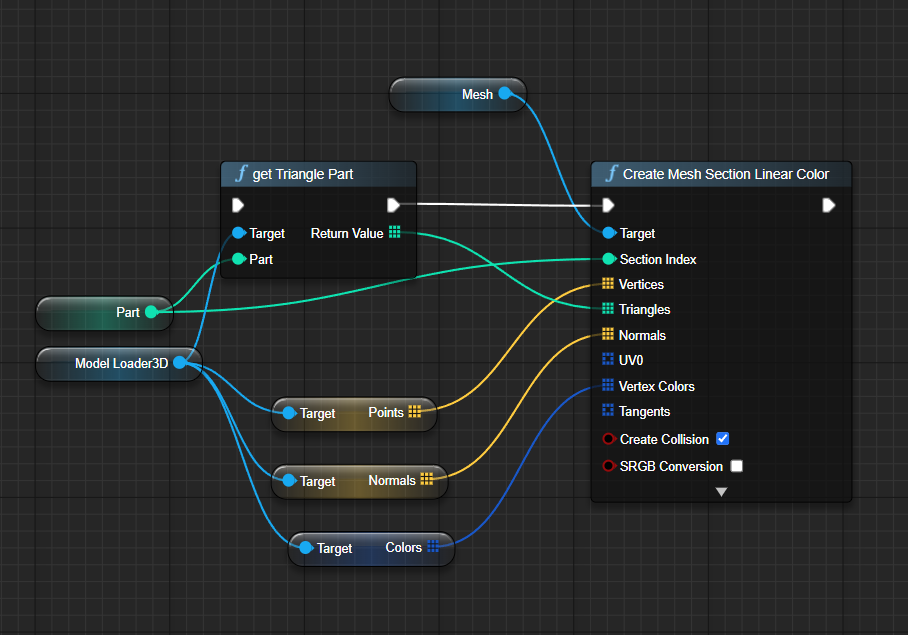
\includegraphics[width=\textwidth]{blueprints/loadingMesh.png}
    \caption{Loading mesh funcion}
    \label{fig:loadingMesh}
\end{figure}
\noindent
To load the mesh, I created a recursive function Fig.[\ref{fig:loadingMesh}] that loads each mesh group every 0.5 ms. A delay is necessary because some 3D models are large and can significantly impact performance during loading, and this helps to mitigate that. The function needs to be recursive because \ac{UE} loops do not allow delays within them.
After all the mesh groups are loaded, another similar function is called to change the material and display the 3D mesh colors.
\subsection{3DmodelVewer actor}
\noindent
The \texttt{3DModelActor} is a custom actor designed to facilitate the visualization of 3D heart models that is an extension of \texttt{Grippable Actor}. This actor comprises four primary components. The first component is the Procedural Mesh, which utilizes Unreal Engine's capabilities to generate and display a heart model in real-time. 
The second component is a Loading Indicator \texttt{Sphere} that provides visual feedback during model loading processes informing users about the ongoing operations. In addition, the \texttt{3DModelActor} features a \texttt{Text Component} that displays error messages when issues arise during the loading of the 3D models.\\
The core functionality of the actor is driven by a custom \texttt{Model Loader}, This custom component is responsible for fetching 3D models from the server, parsing the model data, and integrating it into the procedural mesh and it implements the OBJ parser.\\
The \texttt{Model Loader component} can download the 3D Model from the backend thanks to the function httpFileDownload, that thanks to a delegate, can be runned in an asynchronous way thanks to \ac{UE} threads, and then notify when the execution is complete.
Another functionality of \texttt{3DModelActor} is that it can be gripped thanks to its parent Blueprint \texttt{Grippable Actor}.

\lstinputlisting[language=C++, caption=model loader header file, label={code:model loader}, linerange={12-74}, style=cpp]{code/c++/model loader.h}

\paragraph{Resizable functionality}
As specified in the requirements, the 3D models must be resizable. Therefore, the actor needs an event that allows its size to be changed. This event must be an \ac{RPCs} that is executed on the server, ensuring that the action is replicated across all clients.

\section{The VR Character}
\noindent
Thanks to the VRExpansion plugin, we can use the standard \texttt{VRCharater}, this \texttt{Character} has already implemented the online synchronization, and it also has the components for the controllers and camera management.
The controllers can \texttt{grip} any \texttt{Actor} or \texttt{Component} that implements the interface \texttt{VRGrip}, this will be used for  moving the 3D models.
Other than that the \texttt{VRCharater} is an empty blank, and will need to implement some functions for making it fully functional.\\
Here are the main components to develop:

\begin{itemize}
    \item Input management
    \item Widget Interaction
    \item Interaction pointer
    \item Side menu
    \item Grip framework
    \item 3D model size management    
    \item Loading sphere
\end{itemize}

\subsection{Input management}
\noindent
Input in \ac{UE} is managed by two data files: \texttt{Input Action }and\texttt{Input Mapping Context}.
In the next two paragraphs will be addressed how the input works, and then will be used in the various components of \texttt{VRCharater}.

\paragraph{Input Action}
Are files that are used to identify a certain input of the controller, each file should be named after an action more than the input used for making clear what they serve.
For example:\\
For using the \texttt{A} button find in the right controller,
you need to have a file that represents the button,
the necessary settings are: Consume input which allows you to take into account that the input has been served,
and the type of value that in this case will be \texttt{Digital (bool)}.

\begin{figure}[h]
    \centering
    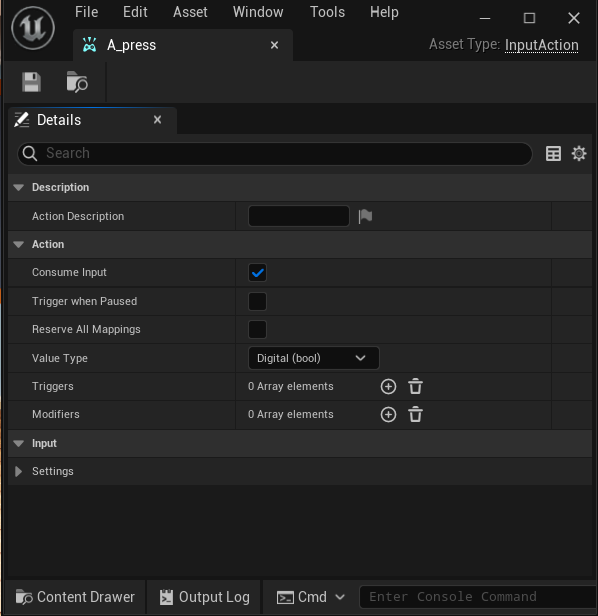
\includegraphics[width=0.7\textwidth]{blueprints/InputActionExample.png}
    \caption{Input Action example}
    \label{fig:InputAction}
\end{figure}

\paragraph{Input Mapping Context}
Files represent all the inputs used by an actor, an actor could change its inputs, so they can be multiple files for different occasions,
Here each \texttt{Input Action} will be associated with the corresponding input.
\texttt{Input Mapping Context} can be used for other objects so that they can override the standard behavior of the \texttt{Character}, for example by equipping a laser pointer and using the \texttt{A} button for toggle it.
Each \texttt{Input Mapping Context} can be bound with different controllers, this can be useful if we will be porting the app for another \ac{HMD}.
For setting the \texttt{Input Mapping Context} there is a function called \texttt{Add Mapping Context}.

\paragraph{Input animations}
Thanks to the rigged 3D models of the controllers provided by Meta, it is possible to import them as \texttt{skeletal meshes}.\\
A \texttt{skeletal} mesh consists of a mesh with an underlying skeleton, allowing it to flex, stretch, or rotate its bones to create animations.
We use these models to animate the controllers, simulating the user's inputs. This allows for visual representation of buttons being pressed, sticks being tilted, and the degree to which triggers and grips are engaged.
These animations are controlled by functions that read the input and adjust the position or rotation of the \texttt{skeletal} mesh bones accordingly.


\subsection{Widget Interaction}
\label{chp:widgetInteraction}
\noindent 
In a normal application we are used to managing input mainly via mouse or touch screens, in \ac{VR} we can not have that, so It's important to create some kind of \ac{UI}.
One of the most used approaches is showing some kind of virtual display with buttons so that the user can interact, for this will be using a blueprint called \texttt{Widget} and will be explained in chapter \ref{sec:widgets}.
Unfortunately \texttt{Widgets} are used for 2D menus but thanks to an actor component we can use it in a 3D environment.\\
For interacting with a \texttt{widget} in a 3D space, \ac{UE} has a component called \texttt{widget interaction} that can evaluate if it is pointing to a \texttt{widget}, it can also give the world location of where it is pointing. This component will be attached to each \texttt{grip motion controller component}.
For letting the user see exactly where the controller is pointed, when the controller is near the \texttt{Widget} a trace will be shown.
For the trace will be used a Component called \texttt{Spline Mesh}, as the name suggests, uses various points and interpolates a mesh for creating a complex curve.
Still our use will be simply by just using two points Fig[\ref{fig:splineExample}]. So the algorithm is simple: each tick a function called \texttt{InteractionPointer} will control both controllers if the \texttt{widget interaction} points to a \texttt{Widget}, then will draw the spline.



\begin{figure}[h]
    \centering
    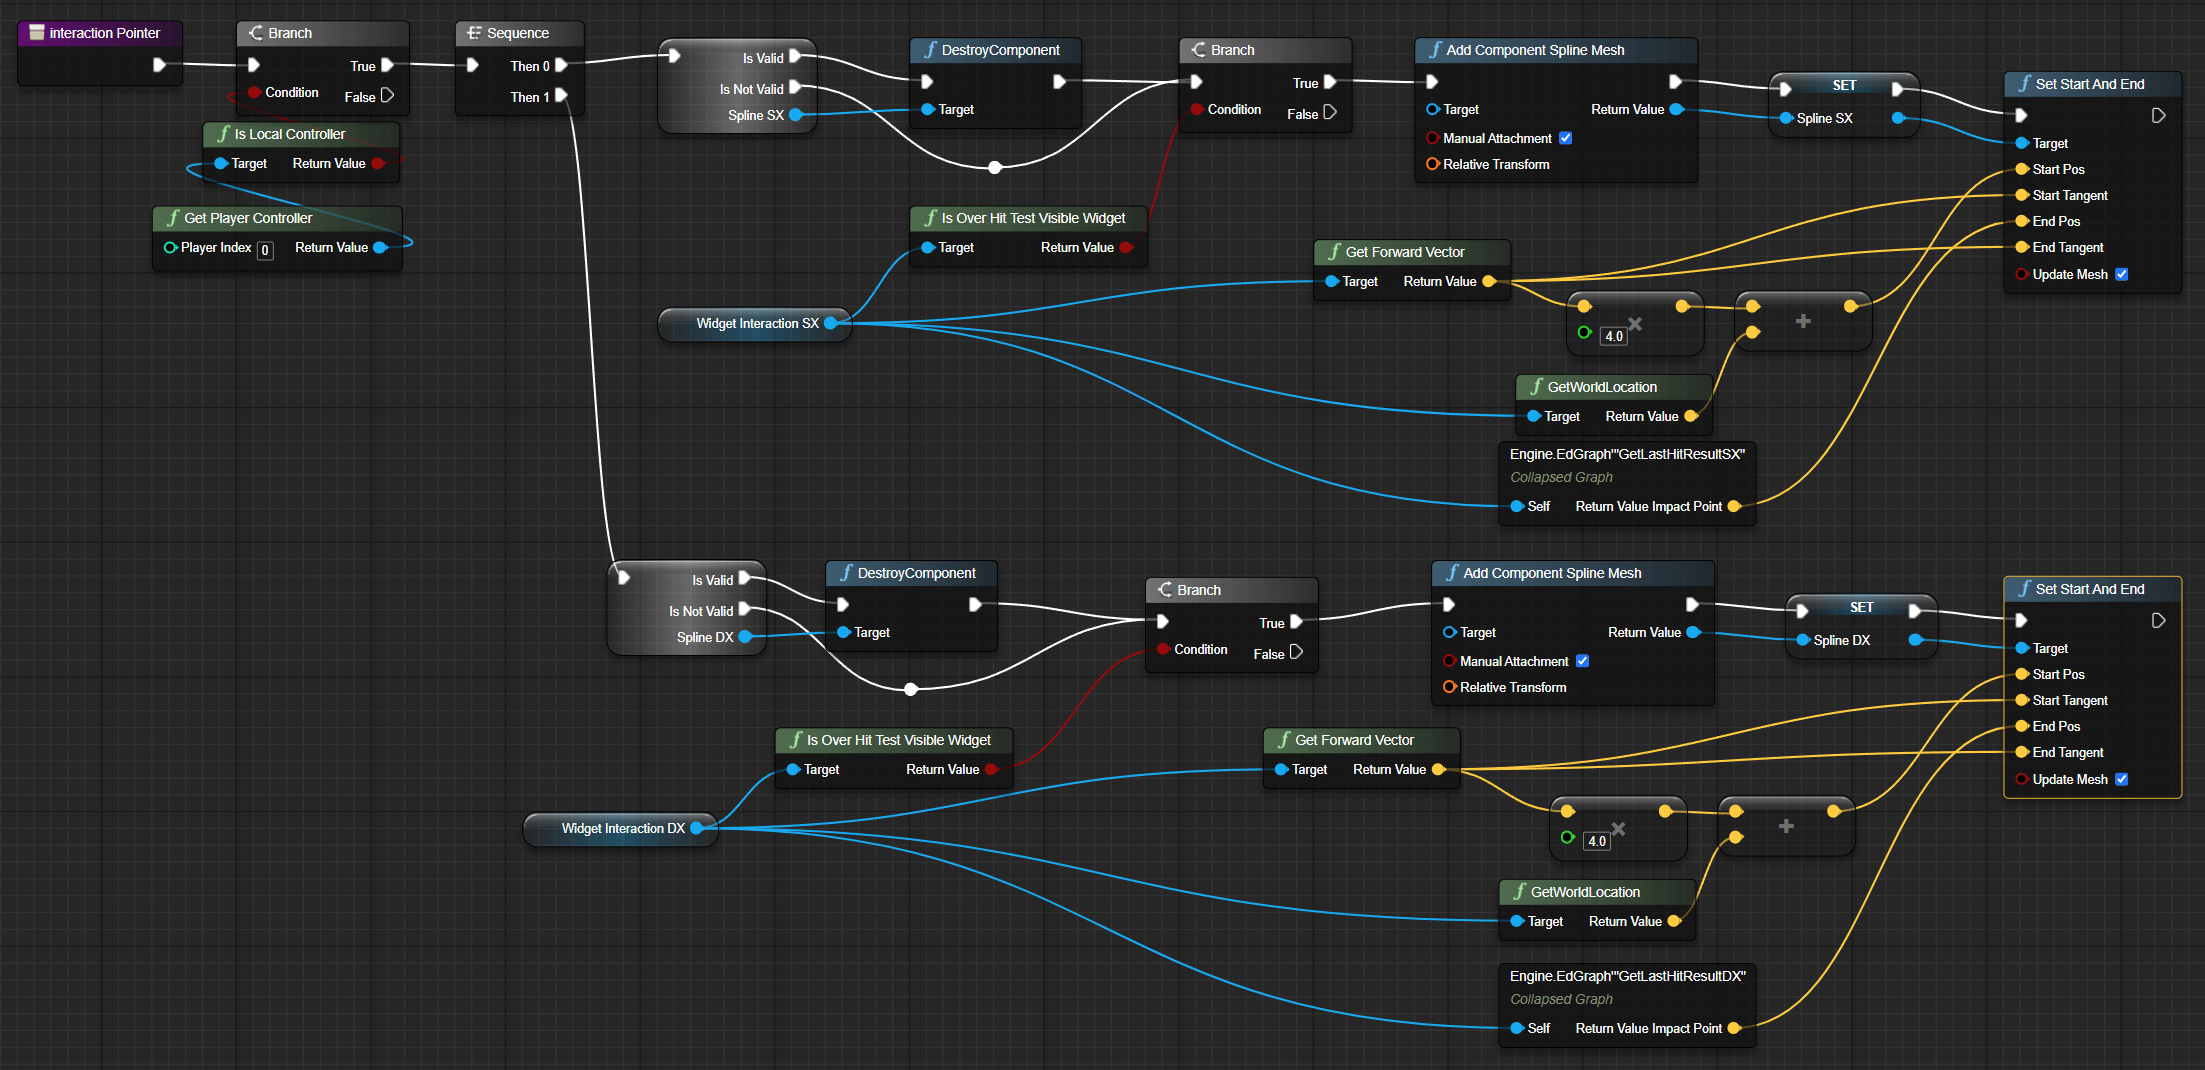
\includegraphics[width=\textwidth]{blueprints/interactionPointer.png}
    \caption{Widget Interaction code}
    \label{fig:InteractionPointer}
\end{figure}

\begin{figure}[h]
    \centering
    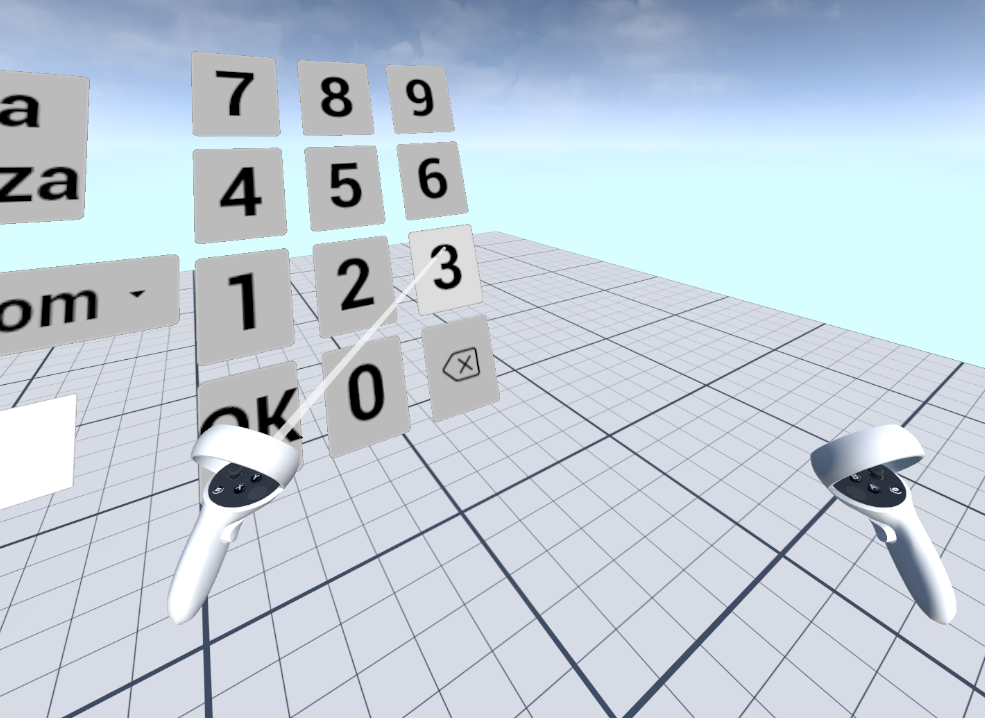
\includegraphics[width=0.8\textwidth]{vrScreenshot/splineExample.png}
    \caption{On the left a controller that create the spline pointing to the widget}
    \label{fig:splineExample}
\end{figure}

\subsection{Laser pointer}
\noindent
To create an effective laser pointer, we can simply use a red spline that starts from the controller and ends on the pointed surface. The code is very similar to the \texttt{widget interaction pointer} described in Chapter [\ref{chp:widgetInteraction}]. However, to find the pointer's location, we can use the line trace function, which detects the nearest point where a geometry intersects with an input segment.\\
The laser pointer will be an actor, and using a component called a child actor, we can attach it to the \texttt{VRCharacter} right controller. This is necessary to eliminate the latency effect caused by the tick group of the \texttt{VRCharacter}, which is set to \texttt{Pre Physic}. The laser pointer actor will stay in the \texttt{post update work}, allowing it to be ticked one frame before anything else.\\
The final result is identical to the \texttt{widget interaction pointer} shown in Fig. [\ref{fig:splineExample}], but the color will be red, and it will be toggled using the \texttt{A button}.

\subsection{Grippable system}
\noindent
Thanks to VRExpansion, we can use a grip function that allows us to attach an actor implementing the \text{VRGripInterface}.
The only challenge is determining which element should be gripped, but \ac{UE} provides a function called Sphere Trace for Objects, which returns the nearest actor within a specified radius.
If the actor implements the \texttt{VRGripInterface}, it can be gripped.\\
The grip is initiated when the controller grip button is pressed, and the object is dropped when the button is fully released.
To avoid conflicts, if both controllers attempt to grip the same object, the object will be dropped when the second controller tries to grip it.

\paragraph{Resizable actor}
For impleming the resizable functionality, all actors that are resizable will implement the \texttt{Resizable actor} interface, that will implement the resizable event.\\
When two controllers will try to grip the same actor, they will drop it, but if both grips are still pressed, the action of moving the controllers closer and further away will allow you to decide the new size of the actor.
For exiting this mode, one controller must relese the grip button.\\
The code for this action is siple, when it's decided that the actior is been resized there the distance between the two controllers will be calculated and the current scale vector of the actor will be saved, afther that the size will be decided by the following formula [\ref{math:ratio}], for smoothness, it will be executed on every tick.

\begin{equation}
    \label{math:ratio}
    New Size=Starting Actor Size \frac{Controllers Distance}{Starting Contrllers Distance}
\end{equation}
    

\section{Widgets}
\label{sec:widgets}
\noindent
Widgets are Blueprints used for creating User interfaces in \ac{UE}, thanks to a lot of pre-made components such as: buttons, textbox, spacers… Each widget can have its own logic built with the Blueprint system.\\
For the app there will be 3 Menus:
\begin{itemize}
    \item \textbf{Main menù:} used for creating a session and joining it. It will have a number pad for inserting the code to enter a session.
    \item \textbf{Side menù:} used as a summable menù that will be displayed over the left controller, used for exiting the session or letting the host use the centering functionality.
    \item \textbf{3d Model picker:} used for selecting what 3D model the host wants to visualize. It will have a dynamically scroll bar section, so that it can load all the names of the models loaded in the server. 
\end{itemize}
\noindent
Unfortunately, widgets are normally used for 2D interfaces, but thanks to an actor component it is possible to visualize them in a 3D space, and is it possible to interact with them thanks to the \texttt{widget interaction component}.\\
Because the menus have to do network calls, they will be able to show error messages and have a loading animation, for cosmetic purposes, the animation will be a schema of a beating heart.


\begin{figure}[h]
    \centering
    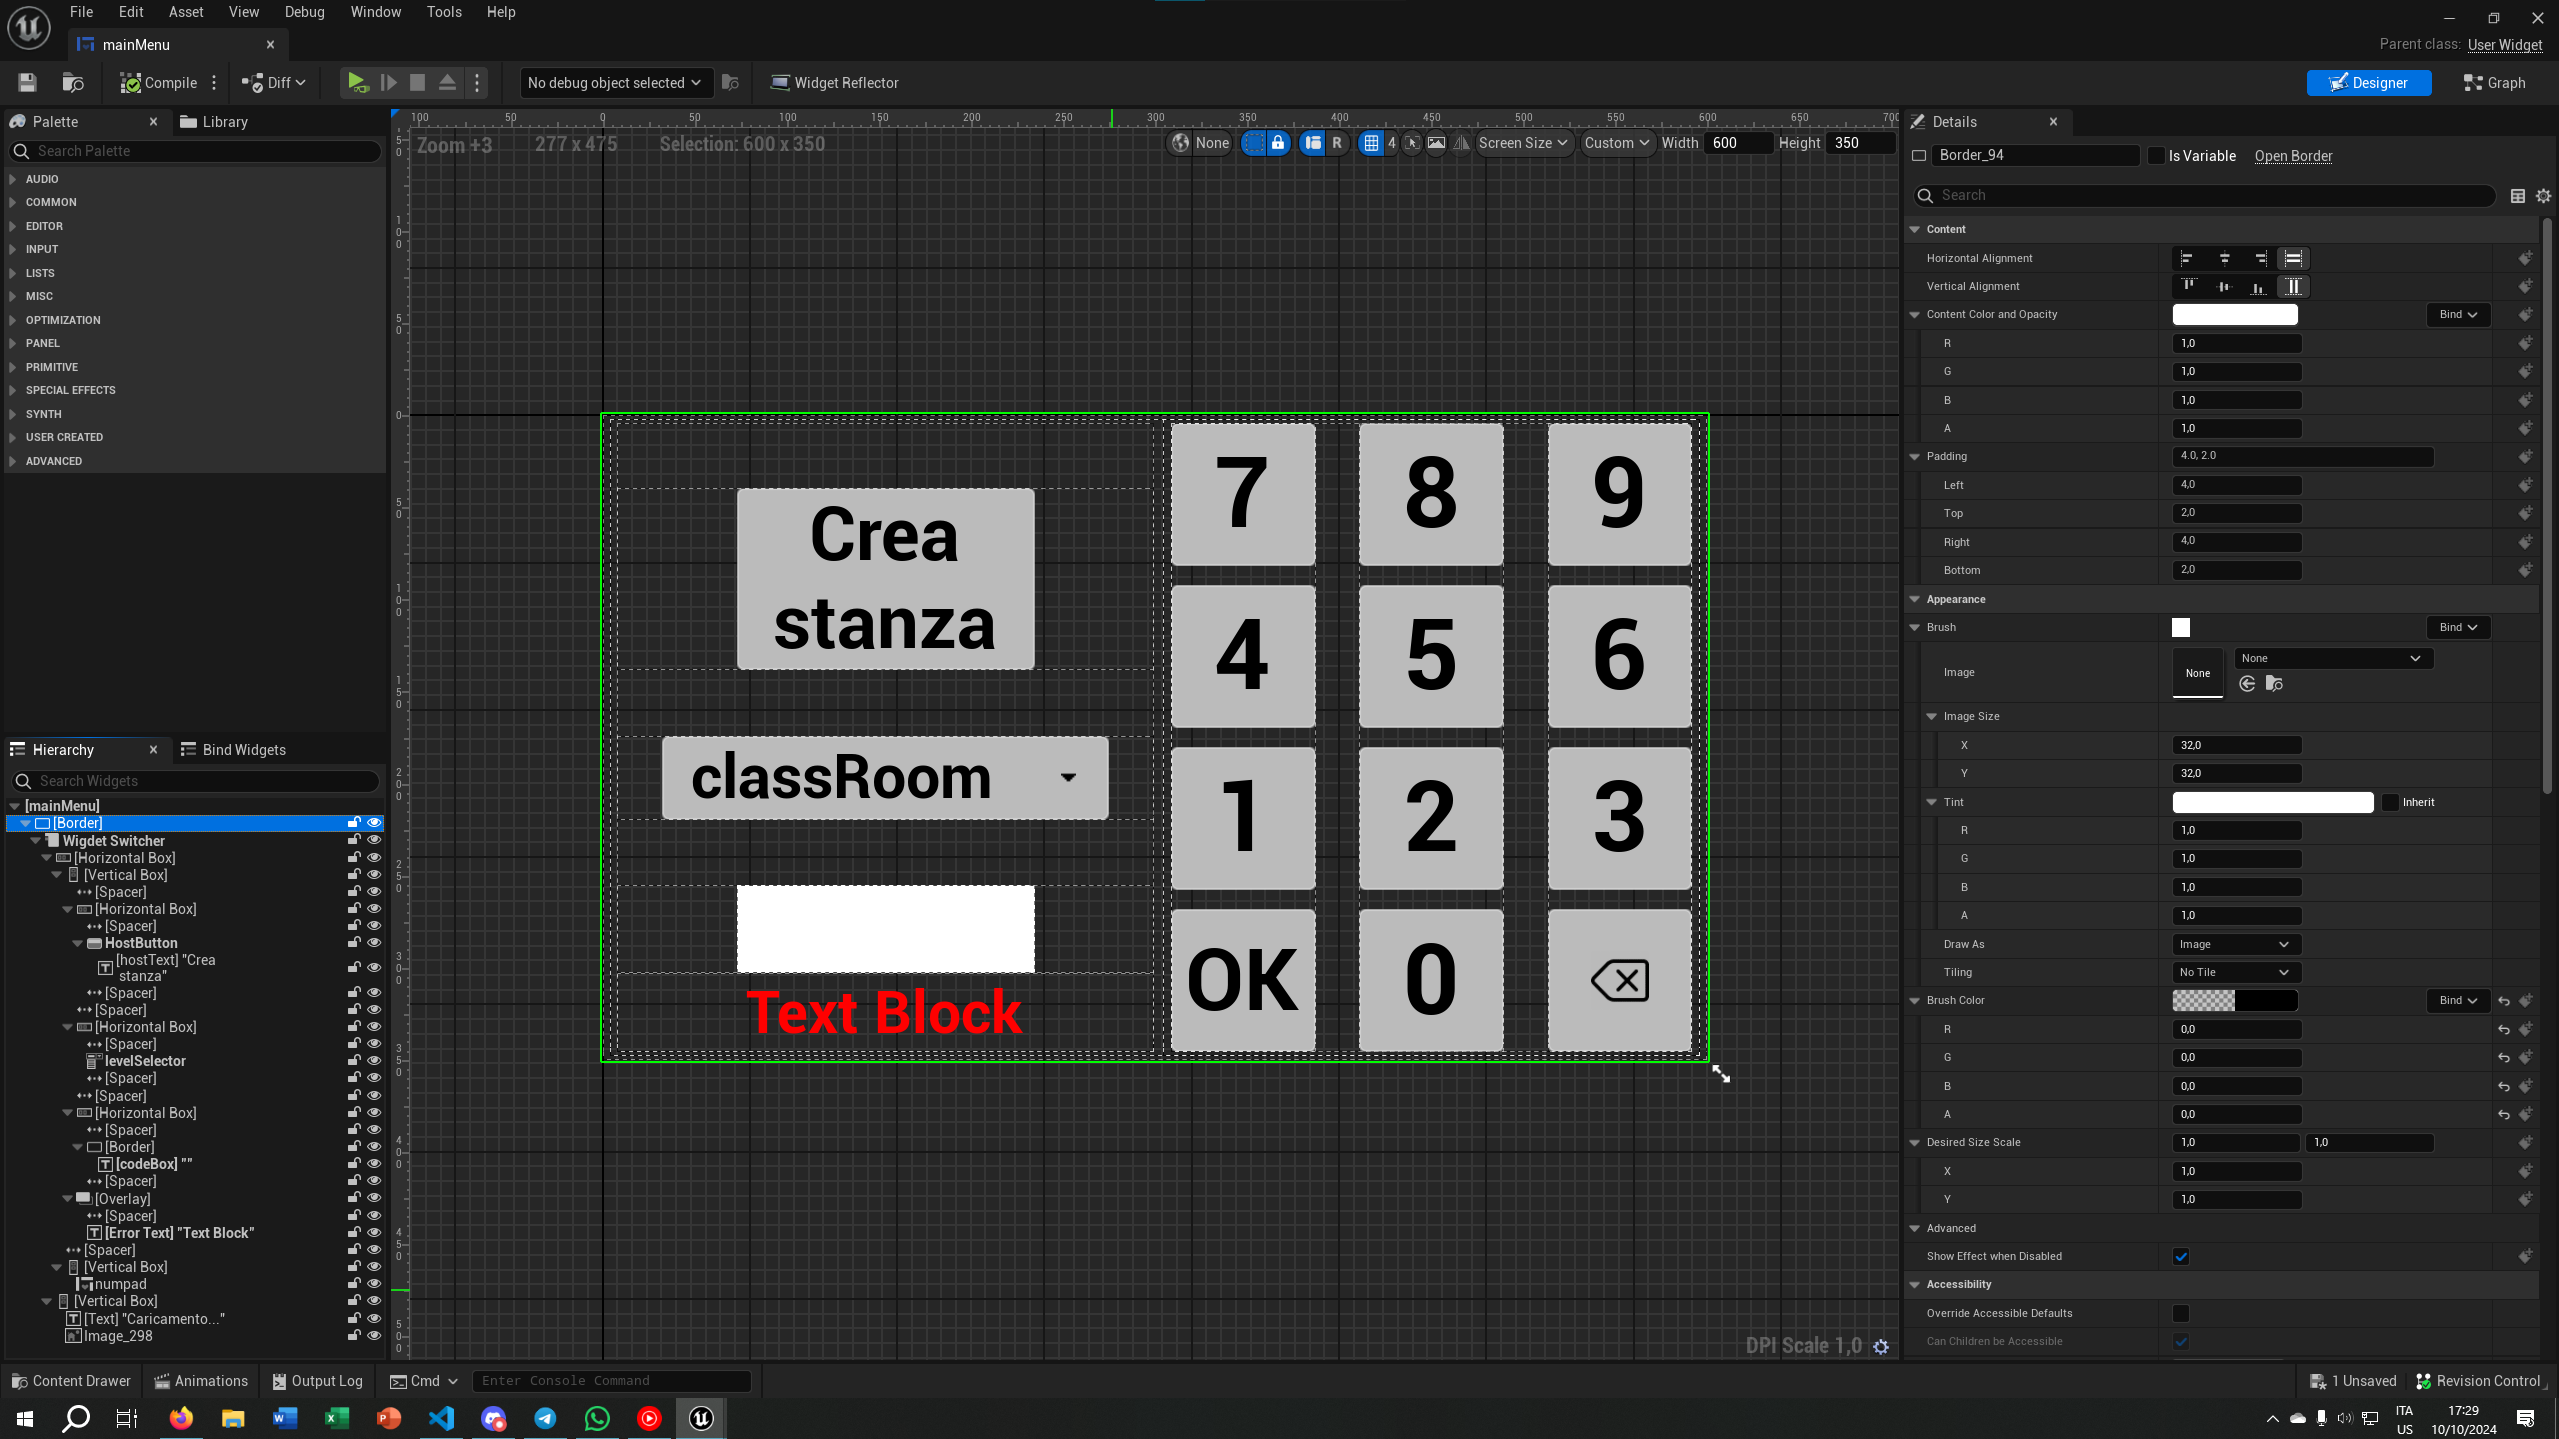
\includegraphics[width=\textwidth]{blueprints/mainMenu.png}
    \caption{Main menu widget}
    \label{fig:mainMenu}
\end{figure}

\subsection{HTTP request}
\noindent
For compatibility reasons with the \ac{HMD}, I built a blueprint function for \ac{HTTP} requests.
Because there is an internet call there is the need to do it in background, fortunately unreal gives a special \texttt{C++} class called \text{UBlueprintAsyncActionBase},
if we inherit it, we can create what in \ac{UE} is called \texttt{latent node} Fig[\ref{fig:HTTPrequest}], these nodes can activate their output pins without stopping the frame until they are complete. 

\begin{figure}[h]
    \centering
    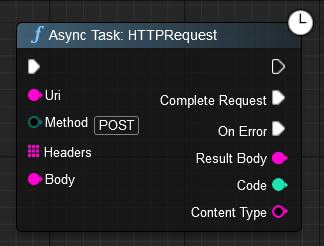
\includegraphics[width=0.4\textwidth]{blueprints/httpRequest.png}
    \caption{HTTP request node}
    \label{fig:HTTPrequest}
\end{figure}
\noindent
Because the app does not need a full \ac{HTTP} implementation we will implement the block with this parameters an outputs:
\begin{itemize}
    \item POST and GET methods using an enumeration
    \item the request headers will be in array of strings
    \item the request body will be of string type
    \item the content type response header will be a string type
    \item the response code
    \item Two output pins for knowing if it received a response or there were some kind of network error
    \item The body response will be of string type
\end{itemize}
\noindent
For ease of use there is another class called \texttt{WorldVariables} that inherits \linebreak\texttt{UBlueprintFunctionLibrary} for accessing the server \ac{URL}, this kind of functions are accessible in all Blueprints and \texttt{C++} code.


\section{Multiplayer functionality}
\noindent